\documentclass[12pt,notitlepage]{article}

% Overleaf project:
% https://www.overleaf.com/project/5fdb880ef955c3369964d601

% View-only link:
% https://www.overleaf.com/read/hkybwqtbtvjb

\usepackage{amsmath, amsfonts, amssymb}
\usepackage[svgnames]{xcolor}
\usepackage{datetime2}
\usepackage{epstopdf}
\usepackage[
	colorlinks=true, 
	citecolor={DarkRed}, urlcolor={DarkBlue}, linkcolor={DarkBlue},
]{hyperref}


% 
\usepackage[version=4]{mhchem}

\usepackage{fullpage}

% Paragraph spacing
\usepackage{parskip}

\usepackage{xspace}

\usepackage{graphicx}
\graphicspath{{../images/}}

% Tables (the order matters here)
\usepackage{makecell}
\usepackage{booktabs}
\usepackage{arydshln}

% For editing purposes:
%\usepackage[margin=10pt]{geometry}

% https://latex.org/forum/viewtopic.php?t=10456
\usepackage{titlesec}
\titleformat{\subsubsection}[runin]% runin puts it in the same paragraph
{\normalfont\bfseries}% formatting commands to apply to the whole heading
{\thesubsubsection}% the label and number
{}% space between label/number and subsection title
{}% formatting commands applied just to subsection title
[.]% punctuation or other commands following subsection title


\newcommand{\TODO}[1]{\textrm{\color{red}TODO: #1}}
\input{todomech}


\renewcommand{\d}{\mathrm{d}}

\newcommand{\NOT}{\ensuremath{\mathop{\mathsf{not}}}\xspace}
\newcommand{\AND}{\ensuremath{\mathop{\mathsf{and}}}\xspace}
\newcommand{\OR}{\ensuremath{\mathop{\mathsf{or}}}\xspace}
\newcommand{\XOR}{\ensuremath{\mathop{\mathsf{xor}}}\xspace}

\newcommand{\TEXT}[1]{\quad\text{#1}\quad}
\newcommand{\with}{\text{ $:$ }}

\newcommand{\cbra}[1]{{\color{gray}\ensuremath{#1}}}
\newcommand{\signal}[1]{\ensuremath{\cbra{\langle}\mathrm{#1}\cbra{\rangle}}}
\newcommand{\protein}[1]{\ensuremath{\cbra{(}\mathrm{#1}\cbra{)}}}
\newcommand{\promoter}[1]{\ensuremath{\cbra{[}\mathrm{#1}\cbra{]}}}

% https://tex.stackexchange.com/questions/543953/arrow-with-blunted-end-head-in-math-mode
\newcommand{\act}{\ensuremath{\to}\xspace}
\newcommand{\rep}{\ensuremath{\mathrel{\raisebox{-.3ex}{\rotatebox{90}{\scalebox{1}[1.2]{$\bot$}}}}}\xspace}

\def\[#1\]{\begin{align}#1\end{align}}

% https://tex.stackexchange.com/questions/114113/how-to-label-text-with-equation-number
\newcommand{\eqnum}{\leavevmode\hfill\refstepcounter{equation}\textup{{(\theequation)}}}


\newcommand{\hh}[1]{{\color{Purple}#1}}
\newcommand{\ra}[1]{{\color{Blue}#1}}


\title{ibiocomp project}
\author{RA \& HH}
\date{\today}


\begin{document}

\maketitle




\section{Introduction}

\subsection{The game of 15 sticks}

Rules of the game: %
%
\begin{quote}
	Two players start with 15 sticks
	and alternatingly 
	take 1, 2 or 3 sticks.
	\\
	The last to take a stick loses.
\end{quote}

\TODO{winning strategy, refer to Table \ref{t:logical-playera}}

\ra{[we may change the bibliography style later, but for the moment names are convenient]}

\subsection{General design}

\TODO{bit encoding}

\TODO{players and subtractor}

\TODO{signaling}

\TODO{mention tubes/microfluidics if applicable}

\TODO{manual intervention}


\section{Logical circuits}

\subsection{The players}

\TODO{Table \ref{t:logical-playera}}

In
\cite{NielsenETAL2016}
we find the gates
$
	\ce{r_0} = 
	\mathop{\mathsf{0x0E}}
	(\ce{s_0}, \ce{s_1}, \ce{w_A})
$
and
$
	\ce{r_1} =
	\NOT
	\mathop{\mathsf{0xF6}}
	(\ce{s_0}, \ce{s_1}, \ce{w_A})
$
among those circuits that performed well.
%


%



% Generated in part using
% https://github.com/numpde/ibiocomp/blob/main/code/20201229_LogicalTables/PlayerA.py

% and
	
% https://crcit.net/c/205b0db18f954c4585b3f87d69fced6c
% https://crcit.net/c/84159c89986c4330978603aeace14aa1

% RA, 2020-12-30
	
\begin{table}[hpbt]
\centering

\begin{minipage}{0.3\linewidth}
	\centering
			
	Winning strategy:
	
	{\ }
	
	\begin{tabular}{cccc|c}
		\multicolumn{4}{c|}{Sticks left} & Take \\
		\hline
		15 & 11 & 7 & 3 & 2 \\
		14 & 10 & 6 & 2 & 1 \\	
		13 & 9  & 5 & 1 & 1 \\	
		12 & 8  & 4 &   & 3 \\	
	\end{tabular}
\end{minipage}
%
\qquad
%
\begin{minipage}{0.25\linewidth}
	\centering
	\begin{tabular}{ccc|cc}
		\ce{w_A} &  \ce{s_1} &  \ce{s_0} &  \ce{r_1} &  \ce{r_0} \\
		\hline
		 0 &   0 &   0 &   0 &   0 \\
		 0 &   0 &   1 &   0 &   0 \\
		 0 &   1 &   0 &   0 &   0 \\
		 0 &   1 &   1 &   0 &   0 \\
		 1 &   0 &   0 &   1 &   1 \\
		 1 &   0 &   1 &   0 &   1 \\
		 1 &   1 &   0 &   0 &   1 \\
		 1 &   1 &   1 &   1 &   0 \\
	\end{tabular}
\end{minipage}
%
\qquad
%
\begin{minipage}{0.25\textwidth}
	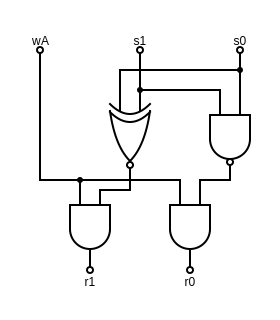
\includegraphics[width=\linewidth]{circuits/Logical-PlayerA.svg.pdf}
\end{minipage}

\caption{%
	Logical circuit for {Player A}.
	%
	The input is a
	wake-up signal \ce{w_A}
	and the bits
	\ce{s_1}/\ce{s_0}
	of the current number of sticks
	(\ce{8 s_3 + 4 s_2 + 2 s_1 + s_0}).
	%
	The output is
	the number of sticks that 
	the player chooses to take,
	encoded as \ce{2 r_1 + r_0}.
	%
	Note that the output is cut off
	when \ce{w_A} is absent.
	%
	%
	The circuit for {Player B}
	is identical except
	that it is controlled up by \ce{w_B}.
}

\label{t:logical-playera}
\end{table}


\subsection{Subtractor} \label{s:sub}

\TODO{Table \ref{t:subtractor1}}

The gates
$
	\ce{c_2} 
%	=
%	\mathop{\mathsf{0x4D}}
%	(\ce{r_1}, \ce{s_1}, \ce{c_1}) 
	=
	\mathop{\mathsf{0x4D}}
	(\ce{c_1}, \ce{s_1}, \ce{r_1}) 
%	=
%	\NOT
%	\mathop{\mathsf{0x8E}}
%	(\ce{r_1}, \ce{c_1}, \ce{s_1})
	=
	\NOT
	\mathop{\mathsf{0x8E}}
	(\ce{c_1}, \ce{r_1}, \ce{s_1})
$,
which are
symmetric in \ce{r_1}/\ce{c_1},
were successfully
implemented in \cite{NielsenETAL2016}.
%
%
However,
we could not find
$
	\ce{d_1} 
	= 
	((\ce{s_1} + \ce{r_1} + \ce{c_1}) \mod 2)
	=
	\mathop{\mathsf{0x69}}
	(\ce{s_1}, \ce{r_1}, \ce{c_1})
	=
	\NOT
	\mathop{\mathsf{0x96}}
	(\ce{s_1}, \ce{r_1}, \ce{c_1})
$,
a.k.a.~there-input \XOR,
explicitly.

%


\TODO{
\ra{Issure:} Can we have a resettable XOR with recombinases
eg as theorized here in Fig.~2g?
\url{https://www.nature.com/articles/s41598-017-07386-3/figures/2}
}


\ra{2-input \XOR with recombinase \cite{BonnetETAL2013}}
\ra{theoretical 3-input Xor with recombinase \cite{ChiuJiang2017}}

\ra{full adder in ``mammalian'' cells \cite{WeinbergETAL2017} (\url{https://www.addgene.org/87552/}),
communicating \cite{AuslaenderETAL2017}}

%




% Generated in part using
% https://github.com/numpde/ibiocomp/blob/main/code/20201229_LogicalTables/Subtractor.py

% RA, 2020-12-30

\begin{table}[hpbt]
\centering

\begin{minipage}{0.2\linewidth}
	\centering
			
	Half-subtractor:
	
	{\ }
	
	\begin{tabular}{cc|cc}
		\ce{s_3} &  \ce{c_3} &  \ce{d_3} &  -- \\
		\hdashline
		\ce{s_2} &  \ce{c_2} &  \ce{d_2} &  \ce{c_3} \\
		\hdashline
		\ce{s_0} &  \ce{r_0} &  \ce{d_0} &  \ce{c_1} \\
		\hline
         0 &          0 &          0 &          0 \\
         0 &          1 &          1 &          1 \\
         1 &          0 &          1 &          0 \\
         1 &          1 &          0 &          0 \\
	\end{tabular}
\end{minipage}
%
\quad
%
\begin{minipage}{0.3\linewidth}
	\centering
			
%		Full subtractor:
%		
%		{\ }
	
	\begin{tabular}{ccc|cc}
		\ce{s_1} &  \ce{r_1} &  \ce{c_1} &  \ce{d_1} &  \ce{c_2} \\
		\hline
         0 &          0 &          0 &          0 &          0 \\
         0 &          0 &          1 &          1 &          1 \\
         0 &          1 &          0 &          1 &          1 \\
         0 &          1 &          1 &          0 &          1 \\
         1 &          0 &          0 &          1 &          0 \\
         1 &          0 &          1 &          0 &          0 \\
         1 &          1 &          0 &          0 &          0 \\
         1 &          1 &          1 &          1 &          1 \\
	\end{tabular}
\end{minipage}
%
\quad
%
\begin{minipage}{0.3\linewidth}
	\begin{align*}
		\ce{& & 8 s_3 + 4 s_2 + 2 s_1 + s_0 &}
		\\
		- \ce{& & 2 r_1 + r_0 &}
		\\
		= \ce{& & 8 d_3 + 4 d_2 + 2 d_1 + d_0 &}
	\end{align*}
\end{minipage}

\caption{%
	The subtractor computes
	\ce{d = s - r} (mod 16).
	%
	Since \ce{r} only has 
	the two lowest bits, 
	a half-subtractor
	is sufficient for
	the bits \ce{d_0}/\ce{d_2}/\ce{d_3}
	and the carry flags \ce{c_1}/\ce{c_3},
	and
	only \ce{d_1}/\ce{c_2}
	require the full subtractor.
	%
	We have $\ce{d_0} = (\ce{s_0} \XOR \ce{r_0});
	\ce{c_1} = \NOT (\ce{s_0} \geq \ce{r_0});
	\ce{d_1} = ((\ce{s_1} + \ce{r_1} + \ce{c_1}) \mathrm{mod} 2);
	\ce{c_2} = \NOT (\ce{s_1} \geq \ce{r_1} \geq \ce{c_1})$.
	%
	%
	See Fig.~\ref{f:logical-subtractor01}
	for a logic circuit of
	the subtractor.
}

\label{t:subtractor1}
\end{table}



The \emph{subtractor} multi-module
keeps track of the number of sticks left.
To appreciate the key design issue, suppose
we manually transmit the response \ce{r_1 r_0 = 01}
of a player
into the medium of the subtractor.
It should compute the new number of the sticks,
yet, it has to do so once
and not keep subtracting the value \ce{r_1 r_0}
that is still present.
One solution is single-use subtractors
but then the result of each computation
has to be imparted to an unused subtractor.
Barring excessive manual intervention,
a feasible design
seems to require some separation of
reading/storing the current state,
computing the new state and communicating it
--
temporally or spatially.
For our purposes
this may include
modest parallelism in extracellular signaling
(but not frequency encoding).
%
%
We propose 
a subtractor composed of two parts A and B,
and
a workflow 
%of Phase A, Interphase, Phase B, Interphase, etc.,
as shown in Table \ref{t:workflow}.
%
Thus,
in Phase A characterized by the supply of 
the signal \ce{w_A},
Subtractor A
emits the current state \ce{s},
Player A responds with \ce{r},
while
Subtractor B
reads \ce{s}/\ce{r}
and
computes the new state % \ce{s} 
{silently}
and remembers the result
to emit it in the next Phase B.
%
The medium is cleared, before
Phase B is initiated by
supplying the signal \ce{w_B}.
%
%
In short,
we require
what could be called
a ``gated memory module''
or
``delayed computation''.
%
Fig.~\ref{f:logical-halfsubtractor0}
illustrates this principle
for the half-subtractor,
cf.~Table~\ref{t:subtractor1}.
%


\begin{table}[hpbt]
	\centering 
	
	% Table made by this script:
	% https://deepnote.com/project/998c51eb-bb3f-4a0f-88e3-c8b50d4d678a#%2Ft_phases.ipynb
	\begin{tabular}{llll}
	\toprule
	{} &                                Phase A &               Interphase &                                Phase B \\
	\midrule
	Experimenter &                        supply \ce{w_A} &  \makecell{clear medium} &                        supply \ce{w_B} \\
	Player A     &                in: \ce{s}, out: \ce{r} &                       -- &                                     -- \\
	Subtractor A &                        out: new \ce{s} &                       -- &  in: \ce{s}/\ce{r}; \makecell{compute} \\
	Subtractor B &  in: \ce{s}/\ce{r}; \makecell{compute} &                       -- &                        out: new \ce{s} \\
	Player B     &                                     -- &                       -- &                in: \ce{s}, out: \ce{r} \\
	\bottomrule
	\end{tabular}
		
	\TODO{caption}
	
	\caption{%
		Workflow.
	}
	
	\label{t:workflow}
\end{table}  

asdfasdfalsdf


\section{Genetic toolbox}


\TODO{mention 3-input boolean functions \cite{NielsenETAL2016}}

\TODO{ribocomputing OR and big AND gates \cite{GreenETAL2017}}

\TODO{Specify initial conditions}


\subsection{Transducers}


\subsubsection*{AmtR}

The TetR family member AmtR is 
the central regulator of nitrogen starvation response
in 
the Gram-positive bacterium
\emph{Corynebacterium glutamicum}
\cite{JakobyETAL2000}.
%
This repressor is released
by
the trimeric adenylylated $\mathrm{P_{II}}$-type 
signal-transduction protein GlnK
\cite{BeckersETAL2005, SevvanaETAL2017},
which is present upon
nitrogen starvation. 
%
The AmtR box and the regulon is 
characterized in 
\cite{BeckersETAL2005},
and
several variants are compared 
in \cite{MuhlETAL2009}.
%
%
\TODO{Do we need (to take care of) the GlnK release mechanism?}
%
It seems clear that 
AmtR sits on the DNA as a dimer
\cite{SevvanaETAL2017},
\cite[\S3.4.2]{Schwab2019}.
%
%
We therefore assume
the mechanism
\begin{subequations}
\[
	\ce{
		2 \protein{AmtR} + \promoter{AmtR}
		& <=>>
		\protein{AmtR}_2 \with \promoter{AmtR}
	}
	%
	\\
	%
	\ce{
		\promoter{AmtR} 
		& ->
		\promoter{AmtR} + \protein{Output}
	}
\]
\end{subequations}
and
the kinetics:
\begin{subequations}
\[
	\label{e:AmtR_Act}
	%
	\promoter{AmtR} 
	& =
	\frac{1}{1 + k_{\ref{e:AmtR_Act}} \protein{AmtR}^{n_{\ref{e:AmtR_Act}}}}
	\promoter{AmtR}_\text{total}
	%
	% here, k = forward / backward
	%
	,
	\\
	%
	\label{e:AmtR_Out}
	%
	\tfrac{\d}{\d{t}}
	\protein{Output} 
	& =
	k_{\ref{e:AmtR_Out}}
	\promoter{AmtR}
	.
\]
\end{subequations}
%
%

% Further literature
%\cite{MuhlETAL2009}
%\cite{BuchingerETAL2009}

\ra{working on this}


\subsubsection*{...}


\subsection{Sensors}

\TODO{Explain intercellular signaling pathways from \cite{DuETAL2020}}

\subsubsection*{3OC6-HSL/LuxR}

Pathway:
\[
	\signal{3OC6\text{-}HSL} \act \protein{LuxR} \act \promoter{Lux} \act \protein{Output}
	.
\]

 
The transcription activator \protein{LuxR}
occurs in Gram-negative bacteria
such as \emph{Vibrio fischeri}.
%
The bacterium is permeable to the (auto)inducer,
here \signal{3OC6\text{-}HSL}.
%
The inducer binds to the N-terminal of \protein{LuxR},
which otherwise inhibits its
functional C-terminal \cite{StevensDolanGreenberg1994}.
%
%
The purified C-terminal binds 
upstream of the \emph{lux} box 
(which is centered at $-42.5$bp \cite{EglandGreenberg1999});
however, 
together with the RNA Pol,
it protects the \emph{lux} box and the \emph{lux} operon
promoter
\cite{StevensDolanGreenberg1994}.
%
%
%
We abbreviate
$\protein{LuxR^\star} := \signal{3OC6\text{-}HSL} \with \protein{LuxR}$
and
$\promoter{Lux^\star} := \protein{LuxR^\star} \with \promoter{Lux}$.
%
%\TODO{
%Let $\protein{LuxR^\star}$ denote 
%the activated form
%$\signal{3OC6}:\protein{LuxR}$.
%}
%
%
We assume the mechanism:
%
\begin{subequations}
\[
	\ce{
		\signal{3OC6\text{-}HSL} + \protein{LuxR}
		& <=>>
		\protein{LuxR^\star}
	}
	\\
	\ce{
		\protein{LuxR^\star} + \promoter{Lux}
		& <=>>
		\promoter{Lux^\star}
	}
	\\
	\ce{
		\promoter{Lux^\star}
		& ->
		\promoter{Lux^\star} + \protein{Output}
	}
	.
\]
\end{subequations}
%
%=======
%	\protein{LuxR^\star} + \protein{RNApol} + \promoter{P_{Lux}}
%	& \longleftrightarrow
%	\protein{LuxR^\star} + \protein{RNApol} : \promoter{P_{Lux}}
%	\\
%	\protein{RNApol} : \promoter{P_{Lux}}
%	& \longrightarrow
%	\protein{RNApol} + \promoter{P_{Lux}} + \protein{Output}
%>>>>>>> c8a0f57bdb0a7b80747263819cbb64562e087765
%\TODO{
%\[
%	\signal{3OC6} + \protein{LuxR}
%	& \longleftrightarrow
%	\protein{LuxR^\star}
%	\\
%	\protein{LuxR^\star} + \protein{RNApol} + \promoter{Lux}
%	& \longleftrightarrow
%	\protein{LuxR^\star} + \protein{RNApol} : \promoter{Lux}
%	\\
%	\protein{RNApol} : \promoter{Lux}
%	& \longrightarrow
%	\protein{RNApol} + \promoter{Lux} + \protein{Output}
%\]
%}
% https://chem.libretexts.org/Bookshelves/Biological_Chemistry/Supplemental_Modules_(Biological_Chemistry)/Enzymes/Enzymatic_Kinetics/Sigmoid_Kinetics
%
%
%
and the kinetics:
%
\begin{subequations}
\[
	\label{e:LuxR_Act}
	%
	\protein{LuxR^\star} 
	& =
	\frac{
		\signal{3OC6\text{-}HSL}
	}{
		k_{\ref{e:LuxR_Act}} + \signal{3OC6\text{-}HSL}
	}
	\protein{LuxR}_\text{total}
%	\TEXT{initially}
%	\protein{LuxR^\star} = 0
	,
	%
	\\
	%%
	\label{e:P_Lux_Act}
	%
	\promoter{Lux^\star} 
	& =
	\frac{
		\protein{LuxR^\star}
	}{
		k_{\ref{e:P_Lux_Act}} + \protein{LuxR^\star}
	}
	\promoter{Lux}_\text{total}
%	\TEXT{initially}
%	\promoter{Lux^\star} = 0
	,
	%
	\\
	%
	\label{e:P_Lux_Out}
	%
	\tfrac{\d}{\d{t}}
	\protein{Output}
	& =
	k_{\ref{e:P_Lux_Out}} \promoter{Lux^\star}
	.
\]
\end{subequations}
%
%
In combination, we have
\[
	\tfrac{\d}{\d{t}}
	\protein{Output}
	=
	k_{\ref{e:P_Lux_Out}}
	\promoter{Lux}_\text{total}
	\frac{
		\signal{} \protein{}_\text{total}
	}{
		k_{\ref{e:LuxR_Act}} k_{\ref{e:P_Lux_Act}}
		+
		k_{\ref{e:P_Lux_Act}} \signal{}
		+
		\signal{} \protein{}_\text{total}
	}
	.
\]


\subsubsection*{Salicylate/NahR}

Pathway:
%
\[
	\signal{Sal} \act \protein{NahR} \act \promoter{Sal} \act \protein{Output}
	.
\]

%

According to 
\cite{SchellWender1986, HuangSchell1991},
the transcription activator \protein{NahR}
binds to the recognition site of \promoter{Sal} at
$-83$ to $-45$,
and does so without the inducer \cite[p.10837]{HuangSchell1991}.
The \protein{NahR} hence activate the expression of \promoter{Sal}.
%
%
%
In \cite{SchellBrownRaju1990},
it was suggested 
that the active configuration of \protein{NahR} is a tetramer,
while \cite{ParkLimShin2005}
reported that 
there could be three different complexes
%
$\protein{NahR} \with \promoter{Sal}$.

\TODO{make coherent}

\hh{
Nevertheless, the configuration changes 
then promotes the RNA polymerase binding near $-35$ (upstream of \promoter{Sal}).
%
%
The inducer
(here \signal{Sal}) can induce the conformation change of \protein{NahR},
and activates the promoter \promoter{Sal}.
}

%
%
Following \cite{Peking2013},
we suppose
that 
$4 \times \protein{NahR}$ bind to the DNA,
and
transcription starts
once
one $\signal{Sal}$
binds to each \protein{NahR}.
%
For the sensors we assume an abundance
of \protein{NahR}
\TODO{describe constitutive promoter},
hence the inactive form of the promoter
is $\protein{NahR}_4 \with \promoter{Sal}$.
%
%
We write
$
	\promoter{Sal^\star} :=
	\signal{Sal}_4 \with \protein{NahR}_4 \with \promoter{Sal}
$
for the active form.
%
%
We assume the mechanism
%
\begin{subequations}
\[
	\ce{
		\signal{Sal} + 
		\signal{Sal}_{k - 1} \with \protein{NahR}_4 \with \promoter{Sal}
		& <=>>
		\signal{Sal}_k \with \protein{NahR}_4 \with \promoter{Sal}
	}
	,
	\quad \text{k} = 1, 2, 3, 4,
	%
	%
	\\
	%
	%
	\ce{
		\promoter{Sal^\star}
		&
		->
		\promoter{Sal^\star} + \protein{Output}
	}
\]
\end{subequations}
%
%Mechanism (here \protein{NahR^\star} denotes the activated (tetramer) form):
%\[
%	\signal{Sal} + \protein{NahR}
%	& \longleftrightarrow
%	\protein{NahR^\star}
%	 \\
%	 \protein{NahR^\star} + \protein{RNApol} + \promoter{P_{Sal}}
%	& \longleftrightarrow
%	\protein{NahR^\star} + \protein{RNApol} : \promoter{P_{Sal}}
%	\\
%	\protein{RNApol} : \promoter{P_{Sal}}
%	& \longrightarrow
%	\protein{RNApol} + \promoter{P_{Sal}} + \protein{Output}
%	.
%\]
%
%
which we implement as:
%
\begin{subequations}
\[
	\label{e:NahR_Act}
	%
	\promoter{Sal^\star}
	& =
	\frac{
		\signal{}^{n_{\ref{e:NahR_Act}}}
	}{
		k_{\ref{e:NahR_Act}} + \signal{}^{n_{\ref{e:NahR_Act}}}
	}
	\promoter{Sal}_\text{total}
	,
	%
	%
	\\
	%
	%
	\label{e:NahR_Out}
	%
	\tfrac{\d}{\d{t}}
	\protein{Output}
	& =
	k_{\ref{e:NahR_Out}} 
	\promoter{Sal^\star}
	.
\]
\end{subequations}



\subsubsection*{pC-HSL/rpaR}

Pathway:
%
\[
	\signal{pC} \act \protein{RpaR} \act \promoter{rpa}
	\act 
	\protein{Output}
	.
\]

\hh{
The p-coumaroyl-HSL -- RpaR system 
(\signal{pC\text{-}HSL})
works similarly to AHL/LuxR
\TODO{use `protein`?}.
%
However, as they come from an anoxygenic phototrophic soil bacterium strain, 
the luxIR-type pair, rpaI and rpaR shows good orthogonality to many
QS signals in use \cite{SchaeferETAL2008}.
}

\ra{
The \emph{Rhodopseudomonas palustris} transcriptional regulator
\protein{RpaR},
when purified,
binds an inverted repeat element 
centered at $-48.5$bp
of its promoter
\cite{HirakawaETAL2011}.
%
%
Transcription depends on 
the inducer 
\emph{p}-coumaroyl-homoserine lactone,
or \signal{pC} for short.
%
%
%There is
%pC-HSL-RpaR-activated antisense transcription of \protein{rpaR}.
%
%
The complex 
$\signal{pC} : \protein{RpaR}$
bound to the promoter
activates transcription
\cite[Discussion]{HirakawaETAL2011}.
}


\subsubsection*{XX}



\subsubsection*{XX}

\ra{--}

\subsubsection*{XX}



\subsubsection*{XX}




\subsection{Recombinases}

\subsubsection*{Bxb1}


Bxb1 gp35/gp47
serine-integrase/excisionase
(Int/Xis)
pair
directs the infection cycle of Bxb1 
in
\emph{Mycobacterium smegmatis}.
%
Stoichiometry, start codons,
degradation rates (proteolysis tags)
and DNA substrate copy number 
were optimized 
in \emph{E.~coli}
in \cite{BonnetSubsoontornEndy2012}
to 
assemble a memory bit
that is
stable and responsive over several generations.
%
A promoter of choice is flanked 
by Int recognition sites
and
its directionality is 
\emph{set}
by Int
and 
\emph{reset}
by Int+Xis.
%
Switching times of $\sim$4h were demonstrated
(but the authors expected 30min to be realistic).
%
\ra{maybe:}
Our convention will be that
the \emph{reset} state corresponds to 
positive output (memory bit is \emph{on}).
%
The final construct
\cite[Fig.~4A]{BonnetSubsoontornEndy2012}
consists of an Int gene 
and
a Xis+Int operon
induced by two separate signals,
which facilitates stoichiometry optimization.
%
However, 
in our design,
an external pulse (say, \signal{w_B}) controls Int,
and
an internal compute unit (say, \ce{s_0 \text{ xor } r_0}) controls Xis.
%
The flanked promoter is activated by another
external signal (say, \signal{w_A}).
%
This achieves the separation 
discussed in \S\ref{s:sub} and Fig.~\ref{f:logical-halfsubtractor0}.

%
% SymBiology:
% https://github.com/numpde/ibiocomp/tree/main/code/20201230_Integrase

%




\subsubsection*{XX}



\subsubsection*{XX}


\subsubsection*{XX}



\section{Simulations}

\subsection{PlayerA}

\url{https://github.com/numpde/ibiocomp/tree/main/code/20201231_SymBio_All/PlayerA}

\TODO{Some details missing:
\href{https://drive.google.com/file/d/1X1uEVNkUiXZqNz7C7m36YjW-g1XctIH0}{click for figure (ignore black part)}}

\subsection{Bit 0}

\url{https://github.com/numpde/ibiocomp/tree/main/code/20201231_SymBio_All/Bit0}

\TODO{this could have the same problem as described in Bit 1}

\subsection{Bit 1}

\url{https://github.com/numpde/ibiocomp/tree/main/code/20201231_SymBio_All/Bit1}


\TODO{\ra{Issue: how to implement this ``Dock'' (and a better name)?}}
\ra{%
Note: This seems similar to
\cite[\href{{https://www.pnas.org/content/pnas/104/8/2643/F1.large.jpg?width=800&height=600&carousel=1}}{Fig.~1}]{WeberETAL2007}.
}
%
Consider bit 1 of Subtractor A.
%
Suppose \ce{s_1 r_1 c_1 = 101},
in which case \ce{c_2 = 0}.
%
Suppose a transcription factor \ce{Y},
which encodes \ce{c_2},
promotes expression of \ce{Xis} in the memory subunit.
%
%
When \ce{w_B} is up,
access to memory is on.
%
Since we want \ce{c_2 = 0},
the amount of \ce{Y} is low,
but
around the timepoint when 
\ce{w_B} is turned off
and the inputs begin to change,
\ce{Y} can experience a transient bump.
%
This is sufficient to produce \ce{Xis}
and thus to cause an unintended \emph{reset}
towards \ce{c_2 = 1}.
%
We found two ways to mitigate this
in the computational model.
%
One is to make expression of \ce{Xis}
conditional on \ce{w_B} also
but this requires that \ce{w_B} goes down
before other change
and could be sensitive to degradation rates.
%
A more robust way
is to introduce a buffer for \ce{Y},
which we call ``Dock'',
that 
%
i)
has high affinity for \ce{Y};
%
ii)
sequesters a large amount of \ce{Y},
about 30x compared to the 
\href{https://en.wikipedia.org/wiki/EC50}{EC50}
of \ce{Y} \act \ce{Xis};
%
iii)
releases \ce{Y} for degradation when \ce{w_A} is up.
%
In this way, 
a transient bump in \ce{Y} is absorbed 
by the Dock,
but a sustained signal 
will overflow the Dock and activate 
transcription of \ce{Xis}.
%


%

\section{Discussion}

\TODO{risks}


\footnotesize
\bibliographystyle{apalike}
\bibliography{refs}


\section*{Appendix}

\TODO{On Figure \ref{f:logical-halfsubtractor0}.}

% https://www.circuit-diagram.org/editor/c/075f8cf9d084400b94f1384cc1c3ba96
\begin{figure}[phbt]
\centering
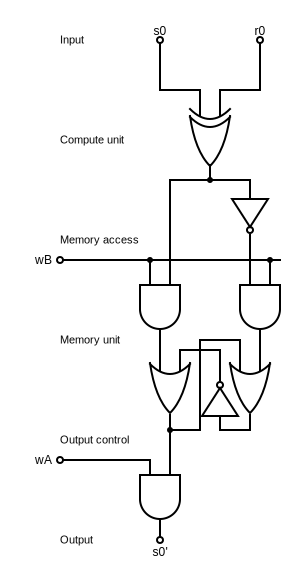
\includegraphics[width=0.5\linewidth]{circuits/Logical-HalfSubtractor0.svg.pdf}
\caption{%
A delayed half-subtractor.
%
The result of the compute unit is written to the memory unit
(bistable switch)
when the signal \ce{w_B} is present.
%
The value of the memory unit is
forwarded to the output
when the signal \ce{w_A} is present.
}
\label{f:logical-halfsubtractor0}
\end{figure}




\clearpage

\SHOWTODOS




\leavevmode\vfill{\tiny\color{lightgray}\hfill{\DTMnow}}
\end{document}





